
\section{Slave Module (SL)}
\label{sec:SL}

The SL module is composed of five modules:

\begin{enumerate}
    \item \mu C Slave (\mu S): transmit measurement data via GSM.
    \item Watchdog Timer (WD): supervise program flow of \mu S.
    \item Voltage Supervisor (SS) : supervise supply voltage of \mu S.
    \item I2C Bus (I2C): implement I2C bus requirements (pullup resistors).
    \item SD-Card Reader (SD): log process data to SD-card.
\end{enumerate}

\begin{figure}[h]
    \centering
    \includegraphics[width=0.9\textwidth]{SL/SL}
\end{figure}



\begin{table}[H]
    \centering
    \begin{threeparttable}[b]
        \begin{tabularx}{\linewidth}{ >{\hsize=0.15\hsize}X >
                    {\hsize=0.15\hsize}X > {\hsize=0.25\hsize}X >{\hsize=3.45\hsize}X}
            Id & Rank & Name             & Net description                                                     \\
            \midrule
            1  & 1    & 3.3V             & regulated voltage provided by \mu S                                 \\
            2  & 4    & \texttt{ESS}     & enable SS                                                           \\
            3  & 4    & \texttt{CON}     & H: \mu S I2C bus and \mu M I2C bus are connected                    \\
            4  & 4    & \texttt{ACK}     & H: \mu S  is ready to receive I2C data from \mu M                   \\
            5  & 4    & \neg \texttt{RS} & reset by watchdog timer, voltage supervisor or on-board user button \\
            6  & 4    & \texttt{EWD}     & enable watchdog timer at the end of the startup code                \\
            7  & 4    & \texttt{RWD}     & reset ("kick") watchdog time to prevent a reset of $U_1$            \\
            8  & 4    & \texttt{SDA}     & I2C data                                                            \\
            9  & 4    & \texttt{SCL}     & I2C clock                                                           \\
            10 & 4    & \texttt{CS}      & SPI, Chip select                                                    \\
            10 & 4    & \texttt{MISO}    & SPI, MISO                                                           \\
            10 & 4    & \texttt{MOSI}    & SPI, MOSI                                                           \\
            10 & 4    & \texttt{SCK}     & SPI, SCK                                                            \\
        \end{tabularx}
    \end{threeparttable}
\end{table}

\clearpage
\subsection{\mu Slave Module (\mu S)}

\mu S is a microcontroller that receives measurement data via the I2C bus and uploads this data to a public mqtt broker via
GSM (GPRS).

\subsubsection{Requirements}
Originally, I planed to use only the  \cite{noauthor_arduino_2020} DK to realize the entire application.
It turned out however, that I was unable to put the u-blox GSM module hosted on the DK into low power mode.
While I was able to obtain some power consumption reduction via the Arduino GSM library, this was by far not enough
for a low power application. I decided therefore to split the functionality across two DKs: one who does the actuals water
flow measurement - the master -  and another separate GSM enabled module - the slave -
to perform actual data transmission.
The master would then control the slave power supply such that the slave and the radio module would only draw current
during the relatively short period required for data transmission.
Hence, the requirements for \mu S are:

\begin{enumerate}
    \item bidirectional data flow between master and slave.
    \item GSM/GPRS compatible modem.
\end{enumerate}

The \cite{noauthor_arduino_2020} provides an I2C interface and fulfills both requirements.
Another solution would have been to simply find a UART-compatible radio module (without additional microcontroller).
While this would have resulted in a simpler and more compact circuit, I would have had to adapt the Arduino GSM library or write
one from scratch.

\subsubsection{Implementation}
\begin{table}[H]
    \centering
    \begin{tabularx}{\linewidth}{>{\hsize=0.25\hsize}X
            >{\hsize=1\hsize}X >{\hsize=1\hsize}X
            >{\hsize=0.5\hsize}X >{\hsize=2.25\hsize}X}
        Id    & BOM Item                     & Order Code & Package  & Rationale                 \\
        \midrule
        $U_1$ & \cite{noauthor_arduino_2020} &            & DIL (28) & availability, ease of use \\
    \end{tabularx}
    \caption{\mu S - BOM}
\end{table}
\begin{table}[H]
    \centering
    \begin{threeparttable}[b]
        \begin{tabularx}{\linewidth}{ >{\hsize=.15\hsize}X >{\hsize=1.35\hsize}X >{\hsize=1.5\hsize}X }
            Id & Issue                               & Potential solution                          \\
            \midrule
            1  & $U_1$: GMS 3 only, chipset obsolete & select a GSM LTE or LTE-M generation module \\
        \end{tabularx}
    \end{threeparttable}
    \caption{\mu S - Issues}
\end{table}

\clearpage
\begin{figure}[h]
    \centering
    \includegraphics[width=1\textwidth]{SL/uS/uS}
    \caption{\mu S - pin out \cite{noauthor_arduino_2020}}
\end{figure}
\begin{table}[H]
    \centering
    \begin{threeparttable}[b]
        \begin{tabularx}{\linewidth}{ >
                    {\hsize=.25\hsize}X >
                    {\hsize=0.5\hsize}X >
                    {\hsize=.25\hsize}X  >
                    {\hsize=.5\hsize}X >
                    {\hsize=.25\hsize}X  >
                    {\hsize=3\hsize}X
            }
                  & \multicolumn{4}{c}{Pin mapping} &                                                                                                            \\
            \cmidrule(lr){3-6}
            Id    & Net                             & Nb. & Name           & Type               & Function                                                       \\
            \midrule
            $U_1$ & .CON                            & 9   & \texttt{A0}    & \rightharpoonup    & high: connect I2C bus to master (bypass the isolation barrier) \\
            $U_1$ & .ACK                            & 10  & \texttt{D0}    & \rightharpoonup    & high: signal to master that I am ready to receive data         \\
            $U_1$ & .CS                             & 11  & \texttt{D1}    & \rightharpoonup    &                                                                \\
            $U_1$ & EWD                             & 12  & \texttt{D5}    & \rightharpoonup    & enable WD                                                      \\
            $U_1$ & RWD                             & 13  & \texttt{D5}    & \rightharpoonup    & reset WD                                                       \\
            $U_1$ & .MISO                           & 17  & \texttt{D2}    & \leftharpoonup     &                                                                \\
            $U_1$ & .SCK                            & 18  & \texttt{D3}    & \rightharpoonup    &                                                                \\
            $U_1$ & .MOSI                           & 19  & \texttt{D4}    & \rightharpoonup    &                                                                \\
            $U_1$ & .SDA                            & 20  & \texttt{SDA}   & \leftrightharpoons &                                                                \\
            $U_1$ & .SCL                            & 21  & \texttt{SCL}   & \rightharpoonup    &                                                                \\
            $U_1$ & \neg RS                         & 24  & \texttt{RESET} & \leftharpoonup     & pulled down by WD timer or user button in case of timeout      \\
            $U_1$ & \Gnd                            & 25  & \texttt{GND}   & \Gnd               &                                                                \\
            $U_1$ & .3V3                            & 26  & \texttt{VCC}   & $\rightarrow$      & regulated output voltage\tnote{1}                              \\
            $U_1$ & .V\textsubscript{\mu S}         & 27  & \texttt{VIN}   & $\leftarrow$       & input voltage controlled by \mu M                              \\
        \end{tabularx}
    \end{threeparttable}
\end{table}
\clearpage

\subsection{Watchdog Module (WD) }

This module is identical to the one discussed in \ref{sec:WD}.
\subsection{I2C Module (I2C)}

This module consists simply of two pullup resistors as required by the I2C interface specification.
I choose to dedicate a separate module to this simple circuit for a couple of reaons:
\begin{itemize}
    \item There is some discussion on how these resistors should be choosen, dependent on the bus speed (TODO).
    \item There is a lot of documentation available for the I2C bus and I wanted a nice home for this material.
    \item I plan to factor out this module into a standalone library that can be shared amongst many projects.
\end{itemize}

\begin{figure}[h]
    \centering
    \includegraphics[width=0.2\textwidth]{SL/I2C/I2C}
    \caption{I2C pullup resistors}
\end{figure}


\begin{table}[H]
    \centering
    \begin{tabularx}{\linewidth}{>{\hsize=0.25\hsize}X
            >{\hsize=1\hsize}X >{\hsize=1\hsize}X
            >{\hsize=0.5\hsize}X >{\hsize=2.25\hsize}X}
        Id    & BOM Item & Order Code & Package & Rationale                \\
        \midrule
        $R_1$ & 10k      & generic    & 0603    & commonly suggested value \\
        $R_2$ & 10k      & generic    & 0603    & commonly suggested value \\
    \end{tabularx}
    \caption{I2C - BOM}

\end{table}
\subsection{SD-Card Reader Module (SD) }

The SD-Card Reader Module (SD) allows to write debug data to a standard SD-card. All the information listed in
\ref{sec:DP} is made persistent for further analysis.
Doing so via GSM transmission would be too costly both in terms of energy consumption and in service usage fees.

\subsubsection{Requirements}

SD must offer a SPI or UART interface because the I2C bus is already used for master-slave communication.
The operating voltage must be either \SI{3.3}{\volt} or \SI{5}{\volt}.

\subsubsection{Implementation}

We use an Arduino-compatible MicroSD Card shield available on various online retailers.

\begin{figure}[h]
    \centering
    \includegraphics[width=1.0\textwidth]{SL/SD/SD}
    \caption{SD - schematic}

\end{figure}


\begin{table}[H]
    \centering
    \begin{threeparttable}[b]
        \begin{tabularx}{\linewidth}{ >
                    {\hsize=.25\hsize}X >
                    {\hsize=0.5\hsize}X >
                    {\hsize=.25\hsize}X  >
                    {\hsize=.5\hsize}X >
                    {\hsize=.25\hsize}X  >
                    {\hsize=3\hsize}X
            }
                  & \multicolumn{4}{c}{Pin mapping} &                                                 \\
            \cmidrule(lr){3-6}
            Id    & Net                             & Nb. & Name         & Type            & Function \\
            \midrule
            $U_1$ & .SCK                            & 4   & \texttt{D5}  & \rightharpoonup &          \\
            $U_1$ & .MISO                           & 5   & \texttt{D6}  & \rightharpoonup &          \\
            $U_1$ & .MOSI                           & 6   & \texttt{D7}  & \leftharpoonup  &          \\
            $U_1$ & .CS                             & 7   & \texttt{D8}  & \leftharpoonup  &          \\
            $U_1$ & .3V3                            & 8   & \texttt{D8}  & \leftarrow      &          \\
            $U_1$ & \Gnd                            & 10  & \texttt{GND} & \Gnd            &          \\
        \end{tabularx}
    \end{threeparttable}
    \caption{SD - pin mapping}
\end{table}
\clearpage
\subsection{Voltage Supervisor (VS)}

The Voltage Supervisor Module (VS) keeps the \mu S in reset as long as the supply voltage
undershoots or overshoots the recommended operating conditions. When the master switches on
the slave power supply, a certain voltage drop is to be expected due to inrush current.
This drop increases as the battery charge decreases. Furthermore, the drop depends on the
ambient temperature. VS ensures that \mu S does not attempt to boot until
the supply voltage has recovered. Failing to do so could lead to undefined behavior.

\subsubsection{Requirements}

VS must be suitable for \SI{3.3}{\volt} systems.

\subsubsection{Implementation}


\begin{figure}[h]
    \centering
    \includegraphics[width=0.8\textwidth]{SL/VS/VS}
    % \caption{WD - schematic}
\end{figure}

\begin{table}[H]
    \centering
    \begin{threeparttable}[b]
        \begin{tabularx}{\linewidth}{ >
                    {\hsize=.25\hsize}X >
                    {\hsize=0.5\hsize}X >
                    {\hsize=.25\hsize}X  >
                    {\hsize=.5\hsize}X >
                    {\hsize=.25\hsize}X  >
                    {\hsize=3\hsize}X
            }
                  & \multicolumn{4}{c}{Pin mapping} &                                                                                      \\
            \cmidrule(lr){3-6}
            Id    & Net                             & Nb. & Name                          & Type            & Function                     \\
            \midrule
            $U_1$ & .3V3                            & 1   & \texttt{SENSE}                & \leftsquigarrow &                              \\
            $U_1$ & \Gnd                            & 2   & \texttt{GND}                  & \Gnd            &                              \\
            $U_1$ & \neg MR                         & 3   & \texttt{\textoverline{MR}}    & \leftharpoonup  & manual reset                 \\
            $U_1$ & .3V3                            & 4   & \texttt{VDD}                  & \leftarrow      &                              \\
            $U_1$ & CT                              & 5   & \texttt{CT}                   & \leftsquigarrow & adjustable reset  delay time \\
            $U_1$ & \neg RS                         & 6   & \texttt{\textoverline{RESET}} & \leftharpoonup  & reset output open drain      \\
        \end{tabularx}
    \end{threeparttable}
    % \caption{VS - pin mapping}
\end{table}
\begin{table}[H]
    \centering
    \begin{tabularx}{\linewidth}{>{\hsize=0.25\hsize}X
            >{\hsize=0.75\hsize}X >{\hsize=1.5\hsize}X
            >{\hsize=0.5\hsize}X >{\hsize=2\hsize}X}
        Id    & BOM Item                     & Order Code          & FF     & Rationale             \\
        \midrule
        $U_1$ & \cite{noauthor_tps3890_2016} & TPS389033DSER / 235 & WSON/6 &                       \\
        $R_p$ & \SI{10}{\kilo\ohm}           & generic             & 0603   &                       \\
        $C_t$ & \SI{100}{\nano\farad}        & generic             & 0603   & \SI{1}{\second} delay \\
    \end{tabularx}
    \caption{VS - BOM}
\end{table}
\clearpage
\clearpage